\chapter{Radio Driver for Zolertia with the RN2483 module}

% Most of the LoRaWAN features were not implemented or tested since this was out of the scope of this project.

Since the \emph{Zolertia RE-Mote REV-B} don't support \emph{LoRa} out of the
box we have to implement a software driver for the Microchip \emph{RN2483} LoRa
module.

\section{Preliminary work}

Last year \emph{Roald Van Glabbeek} started to work on the \emph{RN2483} module
in the course of his master thesis~\cite{8847137} aiming on doing further
research on \emph{energy efficient lora multihop networks}. For this purpose he
created a \emph{RN2483 Shield} adapted to the pin configuration of the
\emph{Zolertion RE-Mote REV-B} and started a driver implementation for the
Contiki-OS\@. The first part of my work consisted in implementing a reliable
and featurefull radio driver for the \emph{RN2483} module working in the last
version of \emph{contiki-ng}.

\section{RN2483 Module Structure}

Developped by \emph{Microchip} the \emph{RN2483} is a LoRa module working on
433 and 868Mhz band . The module is specically design to work with LoRaWAN
compliant network by including a set of commands specifically designed for
seamless connection with to a \emph{LoRaWAN} network. The module design is
aiming for ease of use over performance and low power.
All communication with the module are done with a \emph{UART} ASCII command
interface making it easy to interact with the module by a human that could be
entering command on a terminal and reading the response back in a human
readable format like in Fig~\ref{fig:pcconn}.

\begin{figure}[H] % TODO More info on axis
\centering
\begin{tikzpicture}[auto, thick]
  \node(pc) [server, label=below:{PC}] {};
  \node(ftdi) [draw, rectangle, right=of pc, right=4cm] {USB to UART Adapter};
  \node(module) [draw, rectangle, minimum size=6mm, right=of ftdi, right=2.5cm] (module) {RN2483 Module};

  \path (pc) edge[<->] node[]{USB Connection} (ftdi) ;
  \path (ftdi) edge[->,bend left] node[text width=1cm, align=center]{TX} (module);
  \path (module) edge[->,bend left] node[text width=1cm, align=center]{RX} (ftdi);
\end{tikzpicture}
\caption{Simple communication with the module scenario\label{fig:pcconn}}
\end{figure}


% Command type division
The module's interface include three types of cammands that enable access to
different functions.

\begin{itemize}
  \item \emph{mac} for the LoRaWAN configurations and control.
  \item \emph{radio} for the low-level radio commands to access the transceiver
    directly without the LoRaWAN interface.
  \item \emph{sys} for the module specific configurations such as the module
    GPIOs state, \emph{sleep}, EEPROM memory access, \ldots
\end{itemize}

\section{Testing Setup}

My testing setup was the same as~\cite{8847137}, I used a Zolertia RE-Mote
Rev-B dev board connected to a RN2483 breakout board and connected them like in
Fig~\ref{fig:schemaconn}.

\begin{figure}[H]
  \centering
  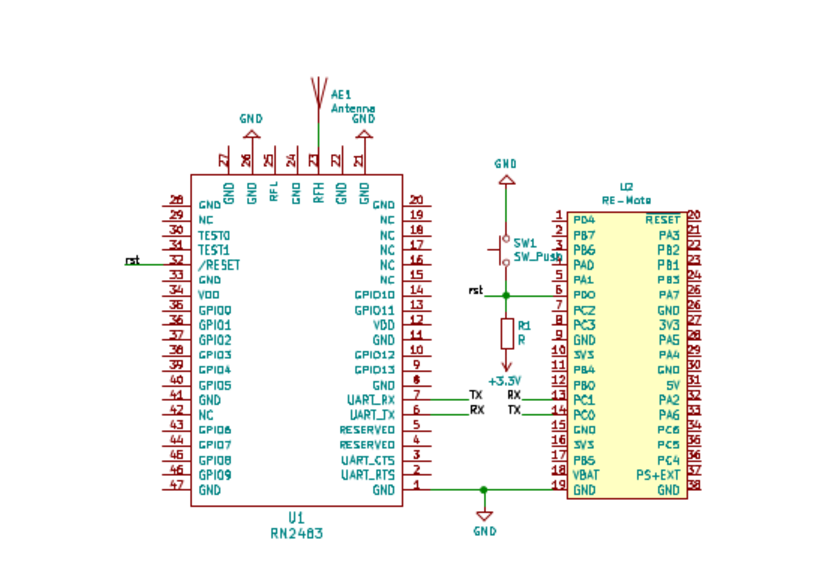
\includegraphics[scale=0.75]{thesis.tex/chapters/driver/fig/conn_diag.pdf}
  \caption{Hardware connection}
  \label{fig:schemaconn}
\end{figure}

\section{Implementation}

\subsection{Structure}

\subsection{Synchronous communication}

\subsection{Contiki Radio Driver}

\section{Validation test}
